\chapter{Методы оценивания декомпозиционной трудности булевых формул в применении к задачам тестирования и верификации логических схем}
\label{ch:partitionings}

% \section{Общие стратегии декомпозиции булевых формул, кодирующих задачи верификации (проверки эквивалентности) логических схем}

% % \todo{Основной вывод: нужно объединять "входы" схем, чтобы уменьшить размерность пространства поиска, а также чтобы получить меньшую дисперсию подзадач.}

% TODO: перенести этот текст в 1 главу (раздел SAT partitioning)

% Для эффективного решения сложных экземпляров SAT часто разумно использовать некоторые техники разделения исходной проблемы на более простые.
% % TODO: fix "partitioning" translation
% Естественным способом декомпозиции экземпляра SAT на подзадачи является так называемый \textit{подход к разбиению} (\textit{partitioning approach})~\cite{hyvarinen2011}.

% Рассмотрим произвольную КНФ-формулу~$C$ над множеством булевых переменных~$X$ и множество $\Pi = \{G_1, \dots, G_s\}$, где $G_i$, $i \in\nobreak \{1, \dots, s\}$, представляют собой некоторые булевы формулы над~$X$.
% Пусть $\Pi$ задает \textit{разбиение}~$C$, если выполняются следующие условия:
% \begin{enumerate}
%     \item формулы $C$ и $C \land (G_1 \lor \dots \lor G_s)$ равновыполнимы (\textit{equisatisfiable});
%     \item для всех $i \neg j \in \{1, \dots, s\}$ формула $C \land G_i \land G_j$ выполнима.
% \end{enumerate}

% Здесь и далее будем называть конъюнкцию произвольных литералов (без эквивалентных и контрарных литералов) из~$X$ как \textit{куб} над~$X$.
% Для произвольной КНФ~$C$ над переменными~$X$ простым примером разбиения является множество $\Pi = \{G_1, \dots, G_{2^r}\}$, которое состоит из всех возможных различных кубов размера~$r$ над множеством~$B$, где $|B| = r$.



% \todo{Описать различные стратегии разбиения: по переменным (входы / (не-)балансные гейты), по кубам (CnC?), по чанкам (объединение входов), по интервалам.}



В данной главе описывается общий подход к оценке трудности примеров SAT, связанных с булевыми схемами, относительно одного класса методов разбиения этих примеров на подформулы.
Такого рода оценка трудности, фактически представляет собой некоторую верхнюю границу сложности рассматриваемой формулы, выраженной в некоторых единицах, которые можно использовать для измерения времени работы полного SAT-решателя.
Также предлагаются две простые конструкции разбиения, которые показали хорошие результаты в вычислительных экспериментах.\\


% ======================================================

\section{Трудность относительно разбиения и вероятностный алгоритм её оценки}

Легко видеть, что можно связать с определенным разбиением SAT $\Pi$ и конкретным полным SAT-решателем~$A$ случайную величину~$\xi_{\Pi}$ так, что общее время работы~$A$ на всех SAT-экземплярах из разбиения~$\Pi$ может быть выражено через математическое ожидание~$\xi_{\Pi}$, которое обозначается как~$\E[\xi_{\Pi}]$.
Этот факт дает теоретические основания для оценки трудности относительно разбиения с помощью простого алгоритма Монте-Карло.

Рассмотрим произвольную КНФ~$C$ над переменными~$X$, и пусть $A$ \=== полный SAT-решатель.
Пусть $\Pi = \{G_1, \dots, G_s\}$ \--- произвольное разбиение~$C$.
Можно рассматривать~$\Pi$ как пространство элементарных событий~\cite{feller1971}, где каждое $G_i$ \--- элементарное событие.
Далее, пусть $p_i$ \=== положительные числа, связанные с каждым~$G_i$ таким образом, что $\sum_{i=1}^{s} p_i = 1$.
Установим $p_i = 1/s$ для каждого $i \in \{1, \dots, s\}$, задав таким образом равномерное распределение на~$\Pi$.
Затем определим случайную величину $\xi_{\Pi} \colon \Pi \to \Real^{+}$ следующим образом:
\begin{equation}\label{f-star}
    \xi_{\Pi}(G \in \Pi) = t_A(G \land C),
\end{equation}
где $t_A(G \land C)$ обозначает время, затраченное~$A$ на определение выполнимости формулы~$G \land C$.

\begin{definition}\label{def:hardness-wrt-part}
    Трудность $C$ относительно алгоритма~$A$ и разбиения~$\Pi$ определяется как значение:
    \begin{equation}\label{eq:hardness-wrt-part}
        \mu_{A,\Pi}(C) = \sum_{i=1}^s t_A(G_i \land C)
    \end{equation}
\end{definition}

\begin{theorem}\label{thm:hardness-wrt-partitioning}
    Справедливо соотношение: $\mu_{A,\Pi}(C) = s \cdot \E[\xi_{\Pi}]$.
\end{theorem}

\begin{proof}%[Набросок доказательства]
    В контексте сказанного выше, имеем вероятностное пространство, где $\Pi = \{G_1,\dots,G_s\}$ \--- пространство элементарных событий, а $\xi_{\Pi}$ \--- определенная на нём случайная величина.
    Пусть $\Spec(\xi_{\Pi}) = \{\xi_1, \dots, \xi_r\}$ ($r \leq s$) \--- спектр $\xi_{\Pi}$, где $\xi_k \in \Real^{+}$, $k \in \{1, \dots, r\}$.
    Обозначим через~$\#\xi_k$ число элементарных событий в~$\Pi$, для которых случайная величина~$\xi_{\Pi}$ принимает значение~$\xi_k$.
    Тогда вероятность события $\{ \xi_\Pi = \xi_k \}$ равна $p_k = \#\xi_k / s$, и $\xi_{\Pi}$~имеет закон распределения $P(\xi_{\Pi}) = \{ p_1,\dots,p_k \}$ (поскольку выполняются все аксиомы Колмогорова~\cite{feller1971}).
    Таким образом:
    \[
        \sum_{i=1}^{s} t_A(G_i \land C)
            = \sum_{k=1}^{r} \#\xi_k \cdot \xi_k
            = s \cdot \sum_{k=1}^{r} \frac{\#\xi_k}{s} \cdot \xi_k
            = s \cdot \E[\xi_{\Pi}]
        \qedhere
    \]
\end{proof}

Используя Теорему~\ref{thm:hardness-wrt-partitioning}, можно оценить $\mu_{A,\Pi}(C)$ с помощью метода Монте-Карло~\cite{metropolis1949}.
Сначала проведем $N$ независимых вероятностных экспериментов, где каждый эксперимент включает выбор $G \in \Pi$ с учетом вероятностного распределения $P = \{p_1, \dots, p_s\}$, с $p_i = 1/s$, где $i \in \{1, \dots, s\}$.
Затем вычислим выборочное среднее~$\xi_{\Pi}$ как $\hat{\mu} = \frac{1}{N} \sum_{j=1}^N \xi^j$, где $\xi^j$ \--- значение~$\xi_{\Pi}$, наблюдаемое в~$j$-ом эксперименте.
Наконец, оценим~$\mu_{A,\Pi}(C)$ как $\widetilde{\mu}_{A,\Pi} = s \cdot \hat{\mu}$.

Будем говорить, что $\widetilde{\mu}_{A,\Pi}(C)$ является $(\varepsilon,\delta)$-приближением~\cite{karp1989} для $\mu_{A,\Pi}(C)$, если выполняется следующее неравенство (вариация условия~\eqref{eq:cheb}):
\begin{equation}\label{eq:cheb2}
    \Pr\Bigl\{
        \bigl|
            \mu_{A,\Pi}(C) - \widetilde{\mu}_{A,\Pi}(C)
        \bigr|
        \leq \varepsilon \cdot \mu_{A,\Pi}(C)
    \Bigr\} \geq 1 - \delta.
\end{equation}
Как следует из неравенства Чебышева, неравенство \eqref{eq:cheb2} выполняется для всех $N \geq \frac{\Var[\xi_{\Pi}(C)]}{\varepsilon^2 \cdot \delta \cdot E[\xi_{\Pi}]^2}$, где $\xi_{\Pi}$ определена относительно \eqref{f-star}.
Однако на практике $\fun{Var}(\xi_{\Pi}(C))$ может быть очень большим, и использование малых значений~$N$ может привести к недостаточной точности оценки~$\mu_{A,\Pi}(C)$.
Эта проблема возникает в таких методах разбиения, как стандартная техника Cube-and-Conquer, а также схема разбиения из~\cite{semenov2021}.
В~следующем разделе представлены две конструкции построения разбиений SAT, которые позволяют уменьшить дисперсию $\Var[\xi_{\Pi}]$ и, следовательно, улучшить точность оценки~$\mu_{A,\Pi}(C)$.



\section{Два новых метода разбиения SAT для CircuitSAT}

В данном подразделе представленны два метода для построения разбиений SAT, нацеленных, главным образом, на задачи из области CircuitSAT.
Соответствующие конструкции могут быть применены как к LEC, так и к задачам обращения криптографических функций.
Ниже приведено описание для LEC.

Рассмотрим задачу LEC для двух булевых схем $S_f$, $S_h$, задающих функции $f,h:\{0,1\}^n\rightarrow{0,1}^m$.
Определим первую конструкцию следующим образом:
\begin{construction}\label{con1}
    Рассмотрим множество переменных $\Xin = \{x_1, \dots, x_n\}$, связанных с входами схем $S_f, S_h, S_{f \glue h}$.
    Затем выберем целое число~$k$ такое, что $1 < k < n$ и разделим~$\Xin$ на~$q = \lceil n / k \rceil$ попарно непересекающихся множеств~$X^j$, где $j \in \{1, \dots, q\}$.
    Если $n$ делится на~$k$, то каждое множество~$X^j$ содержит $k$~переменных.
    В противном случае разделим~$\Xin$ на $q-1$~множества $X^1, \dots, X^{q-1}$ по $k$ переменных каждое и множество~$X^q$ размером~$r$, так что $n = k \cdot \lfloor \frac{n}{k} \rfloor + r$, где $r \in \{1, \dots, k-1\}$.
    % \lipicsEnd
\end{construction}

Рассмотрим произвольную булеву функцию $\lambda \colon \{0,1\}^l \to \{0,1\}$, где~$l \in \Natural^{+}$, и предположим, что $\lambda$~не зафиксирована.
Пусть~$\neg\lambda \colon \{0,1\}^l \to \{0,1\}$ обозначает отрицание~$\lambda$.
С каждым~$X^j$, $j \in \{1, \dots, q\}$, свяжем две КНФ $\phi_1^j$~и~$\phi_2^j$, которые определяют функции $\lambda^j \colon \{0,1\}^{|X^j|} \to \{0,1\}$ и $\neg\lambda^j \colon \{0,1\}^{|X^j|} \to \{0,1\}$ соответственно.
% Следующий факт справедлив.

\begin{theorem}\label{thm:partitioning-input-decomposition}
    Пусть $\phi^j$ обозначает обе формулы $\phi^j_1$~и~$\phi^j_2$.
    Множество~$\Pi$ всех $2^{\lceil n/k \rceil}$ возможных формул вида $\phi^1 \land \dots \land \phi^{\lceil n/k \rceil}$ формирует SAT-разбиение формулы~\eqref{eq:miter-cnf}.
\end{theorem}

\begin{proof}
    Сначала докажем, что формула $C_{f\glue h}$ имеет ровно $2^n$ выполняющих наборов.
    Действительно, рассмотрим множество $X^{in} = \{x_1,\ldots,x_n\}$ и пусть $\alpha=(\alpha_1,\ldots,\alpha_n)$ \--- произвольное назначение переменных из $X^{in}$.
    Затем рассмотрим формулу $\Phi(X,\alpha) = x_1^{\alpha_1} \land \ldots \land x_n^{\alpha_n} \land C_{f\glue h}$ над множеством переменных $X$.
    Из~Леммы~\ref{lem1} следует, что применение UP к~$\Phi(X,\alpha)$ приведет к выводу значений всех переменных из этой КНФ без конфликтов.
    Для каждого $\alpha \in \{0,1\}^n$ построим такое назначение переменных из~$X$ и скажем, что это назначение генерируется соответствующим~$\alpha$.
    Обозначим построенное множество назначений над~$X$ через~$\Lambda(X)$.
    Легко видеть, что все назначения из~$\Lambda(X)$ различны.
    Далее, рассмотрим множество переменных $\tilde{X} = X \setminus X^{in}$.
    С каждым назначением $\lambda \in \Lambda(X)$ свяжем часть~$\lambda$, содержащую назначения переменных из~$\tilde{X}$.
    Обозначим построенное множество назначений как $\Lambda(\tilde{X})$.
    Пусть $\gamma\in\{0,1\}^{|\tilde{X}|}$ \--- произвольное назначение переменных из $\tilde{X}$ такое, что $\gamma\notin \Lambda(\tilde{X})$.
    Очевидно, что подстановка $\gamma$ в $C_{f\glue h}$ приводит к тому, что результирующая КНФ $C_{f\glue h}[\gamma/\tilde{X}]$ является невыполнимой, поскольку для любого $\alpha = (\alpha_1,\dots,\alpha_n)$ применение UP к формуле $x_1^{\alpha_1} \land \dots \land x_n^{\alpha_n} \land C_{f \glue h}[\gamma/\tilde{X}]$ приведет к конфликту.
    Таким образом, любой выполняющий набор $C_{f \glue h}$ \--- это назначение, сгенерированное некоторым $\alpha\in\{0,1\}^{|X^{in}|}$, и различные назначения из $\{0,1\}^{|X^{in}|}$ порождают различные выполняющие наборы~$C_{f \glue h}$.
    Таким образом, у формулы $C_{f\glue h}$ ровно $2^n$ выполняющих наборов.
    С другой стороны, нетрудно видеть, что любое $\alpha \in \{0,1\}^{|X^{in}|}$ выполняет ровно одну формулу $G_i$, $i \in \{1,\dots,2^{\lceil n/k \rceil}\}$ описанного выше вида.
    Таким образом, формулы $C_{f\glue h}$ и $(G_1 \lor \dots G_{2^{\lceil n/k \rceil}})$ имеют одинаковые выполняющие наборы, и, следовательно, формулы $C_{f\glue h}\land C(M)$ и $(G_1 \lor \ldots G_{2^{\lceil n/k \rceil}}) \land C_{f\glue h} \land C(M)$ равновыполнимы.
\end{proof}

Важный вопрос состоит в том, как выбрать функции $\lambda^j$ и $\neg\lambda^j$ таким образом, чтобы гарантировать малую дисперсию $\Var[\xi_\Pi]$ для разбиения SAT описанного выше типа? Здравый смысл подсказывает, что  имеет смысл использовать \textit{сбалансированнаые} булевы функции, т.е. такие функции, которые принимают значение~1 на $2^{l-1}$ входных словах, в качестве функции $\lambda \colon \{0,1\}^l \to \{0,1\}$.
Очевидно, что отрицание сбалансированной функции тоже является сбалансированной функцией. Хорошим примером такого рода функции для $l > 1$ является функция, задаваемая формулой $x_1 \xor \dots \xor x_l$.

Далее проведем несколько неформальный анализ свойств Конструкции~\ref{con1}, и используем его результаты в качестве основы для Конструкции~\ref{con2}, которая показала налучшие результаты среди всех рассмотренных методов в экспериментах с некоторыми чрезвычайно сложными примерами LEC в виде SAT.
Рассмотрим функцию~\eqref{eq:f-glue-h} и шаблонную КНФ~$C_{f \glue h}$.
Многочисленные эксперименты показывают, что даже когда SAT для $C_{f \glue h} \land C(\mathcal{M})$ является чрезвычайно сложной, SAT для~$C_{f \glue h}$ остается простой: любой CDCL SAT-решатель, получив на вход~$C_{f \glue h}$ и не имея никакой дополнительной информации о структуре схемы, способен найти выполняющий набор для~$C_{f \glue h}$.
Этот набор можно рассматривать как сертификат выполнимости для~$C_{f \glue h}$.
Как было отмечено выше, всего для КНФ~$C_{f\Delta h}$ существует $2^n$ таких сертификатов.
Таким образом, доказательство невыполнимости $C_{f \glue h} \land C(\mathcal{M})$ можно рассматривать как процесс, который опровергает все эти сертификаты.
Более того, если функции~$\lambda^j$ сбалансированы для каждого $j \in \{1, \dots, \ceil{n/k}\}$, то каждая формула вида $\phi^1 \land \dots \land \phi^{\ceil{n/k}} \land C_{f \glue h}$ имеет $2^{n - \ceil{n/k}}$ выполняющих наборов, которые также являются сертификатами удовлетворимости.
Таким образом, можно сделать два предположения:
\begin{enumerate}
    \item Алгоритму~$A$ намного легче доказать невыполнимость формулы $\phi^1 \land \dots \land \phi^{\ceil{ n/k }} \land C_{f \glue h} \land C(\mathcal{M})$, потому что ему необходимо опровергнуть $2^{n-\lceil n/k \rceil}$ сертификатов вместо~$2^n$.
    \item Для сбалансированных функций $\lambda^{j}$, $j \in \{1, \dots, \lceil n/k \rceil\}$, все $2^{\lceil n/k \rceil}$ различных формул вида $\phi^1 \land \dots \land \phi^{\lceil n/k \rceil} \land C_{f \glue h} \land C(\mathcal{M})$ должны быть более или менее схожи по времени работы алгоритма~$A$ на них \--- разбиение~$\Pi$, заданное Конструкцией~\ref{con1}, должно иметь малую дисперсию $\Var[\xi_{\Pi}]$.
\end{enumerate}

Хотя представленные аргументы лишены строго формального доказательства, на практике их выводы экспериментально подтверждаются.
Ниже опишем еще одну конструкцию, при разработке которой были учтены указанные выше свойства.

Основная идея описанной ниже конструкции заключается в том, чтобы рассмотреть произвольное назначение переменных из $\Xin =\{x_1,\ldots,x_n\}$ в качестве коэффициентов двоичного представления числа из $N_{0}^{n} = \{0,1,\ldots,2^n-1\}$.
Таким образом, существует взаимно однозначное отображение вида $\{0,1\}^n \to N_{0}^{n}$.
Для произвольных $a,b \in N_{0}^{n}$ назовем множество чисел $\Set{ q \in N_{0}^{n} \given a \leq q \leq b }$ \textit{интервалом} и обозначим такой интервал как~$[a,b]$.
Рассмотрим множество булевых векторов из $\{ 0,1 \}^n$, которые являются двоичными представлениями чисел из~$[a,b]$, как множество решений следующего целочисленного неравенства, предполагая, что $x_i$ принимают значения из~$\{0,1\}$:
\begin{equation}\label{eq-ineq}
    a \leq x_n + 2\cdot x_{n-1} + \dots + 2^{n-1} \cdot x_1 < b
\end{equation}
Скажем, что множество~$\mathcal{R}^n$, образованное интервалами описанного вида, является \textit{полной системой интервалов}, если никакие два интервала из~$\mathcal{R}^n$ не пересекаются и любое число из~$N_{0}^{n}$ принадлежит какому-либо интервалу в~$\mathcal{R}^n$.
Это означает, что любая полная система интервалов порождает разбиение $\{0,1\}^n$ на непересекающиеся подмножества, образованные решениями соответствующих неравенств \eqref{eq-ineq}.

\begin{construction}\label{con2}
    Пусть $\mathcal{R}^n$ \--- полная система интервалов.
    С произвольным интервалом $I = [a,b] \in \mathcal{R}^n$ ассоциируем неравенство вида~\eqref{eq-ineq} и КНФ~$C_I$, полученное путем кодирования~\eqref{eq-ineq} в SAT с использованием соответствующих техник, например, представленных в~\cite{een2006}.
    Определим $\Pi = \{C_I\}_{I \in \mathcal{R}^n}$.
\end{construction}

\begin{theorem}\label{thm3}
    Множество $\Pi = \{C_I\}_{I\in \mathcal{R}^n}$, полученное с использованием Конструкции~\ref{con2}, формирует SAT-разбиение формулы $C_{f\Delta h} \land C(\mathcal{M})$.
\end{theorem}

\begin{proof}%[Набросок доказательства]
    Аналогично доказательству Теоремы~\ref{thm:partitioning-input-decomposition}, используем Лемму~\ref{lem1}, чтобы показать, что любое назначение, удовлетворяющее $C_{f \glue h}$, также удовлетворяет ровно одну формулу вида $G_i \land C_{f \glue h}$, где $i \in \{1, \dots, s\}$.
    Следовательно, можно заключить, что $C_{f \glue h} \land C(\mathcal{M})$ и $C_{f \glue h} \land C(\mathcal{M}) \land {(G_1 \lor \dots \lor G_s)}$ равновыполнимы.
    С~другой стороны, ясно, что любая КНФ вида $G_i \land G_j$ (где $i \neq j \in \{1, \dots, s\}$) невыполнима.
    Значит, $\Pi = \{G_1, \dots, G_s\}$ является SAT-разбиением формулы $C_{f \glue h} \land C(\mathcal{M})$.
\end{proof}

Заметим, что в случае, когда $\mathcal{R}^{n}$ формируется интервалами равного размера~$2^{l}$, где $1 \leq l < n$, можно указать любой интервал $I \in \mathcal{R}^{n}$ без использования кодировок из~\cite{een2006}.
Действительно, в этом конкретном случае интервал с номером $k \in \{ 1, \dots, 2^{n - l} \}$ состоит из чисел вида $(k - 1) \cdot 2^{l} + j$, где $j \in \{ 0, \dots, 2^{l}-1 \}$.
Следовательно, этот интервал можно указать с помощью двоичного вектора $\lambda_{l + 1} \dots \lambda_{n}$, где $\lambda_{q}$ являются коэффициентами из $\{ 0,1 \}$ в двоичном представлении числа ${ (k - 1) \cdot 2^{l} }$ из $n$~бит.

Заметим, что описанный подход не применим к интервалам произвольного вида.
В самом деле, рассмотрим небольшой пример: для $n = 6$ вектор $(010111)$ указывает на число~$23$, а вектор $(101000)$ соответствует числу~$40$.
Тогда, не существует числа $i \in \{ 1, \dots, 6 \}$ такого, что $x_i$ принимает одно и то же значение во всех числах из интервала $[23,40] \subseteq \NaturalZero$.
Поэтому в общем случае необходимо применять техники, такие как например, описанные в~\cite{een2006}, для кодирования интервалов вида~\eqref{eq-ineq} в~SAT.


% \section{Экспериментальное исследование}
% \section{Вероятностный и статистический анализ свойств предложенных разбиений}

% \todo{Вычислительные эксперименты и их результаты}
% \todo{Multipliers, Sorters, Cryptography}
% \todo{Статистические оценки, результаты из IEEE, доверительные интервалы, обоснование мощности выборки}

\section{Вычислительные эксперименты}
\label{sec:experiments}

Все эксперименты, представленные в данном разделе, были проведены на кластере Университета ИТМО, каждый узел которого оснащен двумя 18-ядерными процессорами Intel Xeon E5-2695~v4 и 128~ГБ оперативной памяти.
В качестве SAT-решателя были использованы Kissat\footnote{\url{https://github.com/arminbiere/kissat}} (версия 3.0.0) и CaDiCaL\footnote{\url{https://github.com/arminbiere/cadical}} (версия 1.9.5) из-за их высокой производительности, широких возможностей по настройке и программному взаимодействию через API.
Это было согласовано даже при использовании подхода CnC с инкрементальными решателями (включая те, которые интегрированы в репозиторий CnC и последнюю версию CaDiCaL).
Kissat выделялся при решении кубов на всех тестовых наборах и решателях.

Основным вопросом, который исследовался в вычислительных экспериментах, была точность оценок сложности относительно разбиения (в смысле формулы~\eqref{def:hardness-wrt-part}).
Ситуации, когда сложность относительно разбиения меньше или близка к времени работы последовательного решателя на исходной задаче, являются особенно интересными, потому что в таких случаях соответствующие разбиения позволяют не только точно оценить время решения задачи (в отличие от случая последовательного решения), но и обеспечивают более эффективную стратегию решения соответствующего экземпляра LEC.

% Все дополнительные материалы к настоящей статье доступны онлайн\footnote{\url{https://github.com/Lipen/FMCAD-2023-Supplementary}}.


\subsection{Тестовые данные}

Мы рассматриваем два класса тестовых наборов (бенчмарков).
Первый класс состоит из (невыполнимых) экземпляров задачи LEC для схем, представляющих алгоритмы умножения, такие как
\enquote{умножение столбиком}, \enquote{дерево Уоллеса}~\cite{cormen1990}, \enquote{алгоритм Карацубы}~\cite{knuth-vol2} и \enquote{умножитель Дадда}~\cite{dadda1965}.
Эти экземпляры обозначаются как \instance{AvB}{k}, где \Instance{A} и \Instance{B} означают алгоритмы умножения, а $k$ \=== количество бит в умножаемых числах.
Например, \instance{CvK}{16} представляет собой экземпляр LEC для проверки эквивалентности умножения двух 16-битных чисел (\texttt{16x16} умножитель) методом столбика и алгоритмом Карацубы.
Известно, что такого рода тесты крайне сложны для современных SAT-решателей~\cite{kaufmann2019,semenov2021}.

Второй класс состоит из нескольких (выполнимых) экземпляров, связанных с алгебраическим криптоанализом~\cite{bard2009}, а именно, SAT-кодировок атаки поиска прообраза для хеш-функции MD4 с уменьшенным числом раундов.
Эта проблема была недавно решена в~\cite{zaikin2022} с использованием подхода Cube-and-Conquer.
Набор тестовых примеров на основе MD4 служит для того, чтобы показать, что предложенная техника применима к (1)~выполнимым тестам (2)~тестам не из области LEC.


\subsection{Эксперименты по оценке декомпозиционной сложности}

В первом наборе экспериментов оценивается сложность экземпляров LEC для умножителей относительно предложенных разбиений SAT, где множество входов~$\Xin$ разбивается на непересекающиеся подмножества, называемые \textit{чанками} (\textit{chunks}), в соответствии с Конструкцией~\ref{con1}.
Мы рассматриваем следующие виды функций~$\lambda^j$:
\begin{itemize}
    \item \Part{2-XOR}: $\lambda^1 = x_1 \xor x_2$, \Part{3-XOR}: $\lambda^1 = x_1 \xor x_2 \xor x_3$, \textit{и т.д.};
    \item \Part{2-DIS}: $\lambda^1 = x_1 \lor x_2$;
    \item \Part{3-MAJ}: $\lambda^1 = \fun{majority}(x_1, x_2, x_3)$, где $\fun{majority}(a, b, c) = (a \land b) \lor (a \land c) \lor (b \land c)$;
\end{itemize}
Функции $\lambda^j$ для $j > 1$ определены на соответствующих непересекающихся чанках входов, например, $\lambda^2 = x_4 \xor x_5 \xor x_6$ для \Part{3-XOR}.
Во всех случаях формулы, соответствующие $\lambda_1^j = \lambda^j$ и $\lambda_2^j = \neg\lambda^j$, были закодированы в~КНФ.

Аналогично, для разбиений SAT, построенных в соответствии с Конструкцией~\ref{con2}, используется обозначение~\Part{INT-s}, где $s$~обозначает количество интервалов, например, \Part{INT-65536} соответствует разбиению на \np{65536}~подзадач.

Чтобы обеспечить достоверность и актуальность наших результатов, среди всех составленных бенчмарков были выбраны только те экземпляры, которые представляют практический интерес, то есть те, которые не решаются за несколько секунд, но при этом могут быть решены за разумное время.
Для тестовых наборов алгоритмов сортировки были выбраны экземпляры, которые кодируют LEC для $k = 9$ и~$l = 4$.
Среди умножителей были выбраны экземпляры двух разных уровней сложности (умножители \texttt{12x12} и \texttt{16x16}, например, \instance{CvK}{12} или \instance{KvW}{16}) для демонстрации гибкости нашего подхода в решении задач с различной сложностью.
Для каждого выбранного тестового примера были построены соответствующие разбиения и были решены \textbf{все} подзадачи, чтобы вычислить истинные значения математического ожидания~$\E[\xi_\Pi]$ и дисперсии~$\Var[\xi_\Pi]$.

Кроме того, были рассмотрены разбиения, построенные с использованием техники Cube-and-Conquer (CnC).
Для этой цели были построены кубы с помощью \texttt{march\_cu}\footnote{\url{https://github.com/marijnheule/CnC}}.
В частности, были подобраны значения опций \texttt{-d <depth>} и \texttt{-n <number>} таким образом, чтобы размеры полученных разбиений были аналогичны разбиениям, построенным с помощью методов, предложенных в данной работе.
Для некоторых \enquote{простых} экземпляров также был запущен \texttt{march\_cu} с параметрами по умолчанию, которые могут рассматриваться как базовый уровень в этом экспериментальном исследовании.
Отметим, что для некоторых \enquote{более сложных} тестов \texttt{march\_cu} в режиме по умолчанию не смог выдать результаты (т.е. набор кубов) за разумное время (24~часа), что привело к пропуску этих экспериментов.
Затем все полученные кубы были независимо решены параллельно.
Далее в этом документе будем обозначать разбиения, сгенерированные в идеологии CnC, как \Part{CnC-d*}, \Part{CnC-n*} и \Part{CnC-default}.

\begin{figure}[!htb]
    \centering
    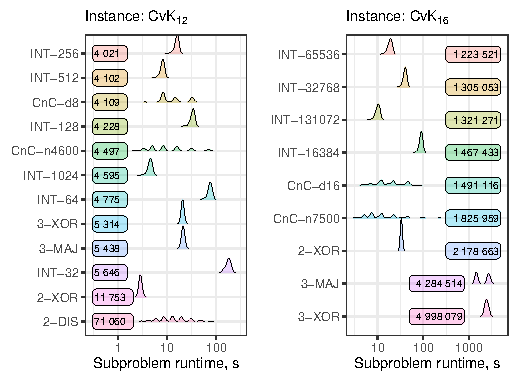
\includegraphics[scale=1.5]{plot_merged-ridges_CvK-12-CvK-16_all-ID-INT-CnC_kissat.pdf}
    \caption{Распределения времени выполнения SAT-решателя на подзадачах в различных разбиениях экземпляров LEC \instance{CvK}{12} (слева) и \instance{CvK}{16} (справа). Цифры рядом с графиками плотности указывают общее время выполнения (в секундах), и все разбиения упорядочены по общему времени (наименьшее время сверху)}
    \label{fig:ridges}
\end{figure}

\begin{table}[p]
    \centering
    \caption{Экспериментальные результаты для SAT-разбиений для задачи проверки эквивалентности (LEC) умножителей}
    \label{tab:results-partitionings-best}
    \subfile{tex/tab-parts-best}
\end{table}

Результаты экспериментов кратко представлены на Рисунке \ref{fig:ridges}~и в Таблице~\ref{tab:results-partitionings-best}.
В~частности, Рисунок~\ref{fig:ridges} содержит
подробные результаты для \textit{всех} обсуждаемых типов разбиений на двух выбранных экземплярах (\instance{CvK}{12} и \instance{CvK}{16}).
В то же время, Таблица~\ref{tab:results-partitionings-best} представляет \emph{лучшие} разбиения для остальных экземпляров.
Для каждого разбиения приводится среднее и стандартное отклонение (\enquote{Avg~$\pm$~sd}), диапазон времени выполнения подзадач (\enquote{Min\,--\,max}) и общее  время (CPU Time), необходимое для решения всех подзадач.
Таблица также включает строки \enquote{Sequential} для представления базовой производительности последовательного решателя SAT.

Графики на Рисунке~\ref{fig:ridges} визуализируют дисперсию времени выполнения SAT-решателя при использовании рассматриваемых схем разбиения.
Для конструкций \ref{con1}~и~\ref{con2} (разбиения \Part{2-XOR} и \Part{INT}, соотвественно) время работы SAT-решателя имеет относительно низкую дисперсию, что указывает на то, что можно точно оценить необходимое общее время выполнения, используя относительно небольшой объем выборки.
Напротив, для Cube-and-Conquer и разбиений \Part{2-DIS} дисперсия значительно больше из-за неравномерного распределения сложности подзадач.
Для последнего это можно объяснить несбалансированностью функции $\lambda = a \lor b$, используемой в \Part{2-DIS}.
Эти результаты подчеркивают важность выбора подходящих схем разбиения для достижения построения точной оценки общего времени выполнения.

Экспериментальные результаты показывают, что оценка для разбиения не всегда согласуется с временем работы последовательного решателя на исходной задаче.
При этом, интересно, что наши результаты показывают, что общее время, необходимое для решения всех подзадач для умножителей, существенно меньше времени, необходимого для последовательного решения соответствующих тестовых примеров.
В частности, для 16-битных умножителей однопоточный решатель не смог завершить работу даже после 10 дней, в то время как все подзадачи в разбиении были решены за разумное и \emph{предсказуемое} время, соответствующее оценке.
Для \enquote{Sequential} строки в таблицах следует уточнить, что решатель работал на одном ядре, в то время как все остальные эксперименты вычислялись параллельно, и представленное общее время CPU является суммой времени работы на всех подзадачах.

\begin{figure*}[!htb]
    % Note: total text width is 43pc, each of 4 subfigures should have width=1.7in
    \centering
    \subfloat[][\instance{CvK}{16}, \Part{2-XOR} / \np{65536}]{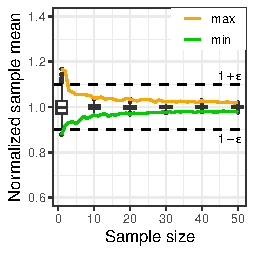
\includegraphics{plot_samples-min-max-boxplots_CvK-16_2-XOR_kissat.pdf}}
    \hfill
    \subfloat[][\instance{CvK}{16}, \Part{INT} / \np{65536}]{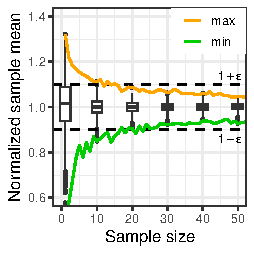
\includegraphics{plot_samples-min-max-boxplots_CvK-16_INT-65536_kissat.pdf}}
    \hfill
    \subfloat[][\instance{CvK}{16}, \Part{CnC-d16} / \np{65536}]{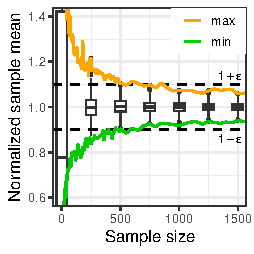
\includegraphics{plot_samples-min-max-boxplots_CvK-16_CnC-d16_kissat.pdf}}
    \hfill
    \subfloat[][\instance{MD4}{40}, \Part{INT} / \np{110000}]{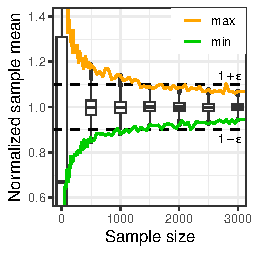
\includegraphics{plot_samples-min-max-boxplots_MD4-40_INT-110000_kissat.pdf}}
    \caption{Распределения выборочных средних для различных размеров выборок~$N$ для экземпляра LEC \instance{CvK}{16} и задачи нахождения прообраза MD4 \instance{MD4}{40}}
    \label{fig:min-max-CvK-16-kissat}
\end{figure*}

В контексте всего сказанного выше, одной из основных проблем является точность полученных оценок~$\E[\xi_\Pi]$, так как дисперсия~$\Var[\xi_\Pi]$ оказывает отрицательное влияние на точность.
Однако результаты в Таблице~\ref{tab:results-partitionings-best} показывают, что предложенные методы SAT-разбиения дают очень низкую дисперсию на рассматриваемых бенчмарках.
Это является значительным преимуществом предложенного метода, так как он позволяет использовать небольшую случайную выборку для получения надежной оценки~$\E[\xi_\Pi]$.
Для демонстрации этого проведем дополнительный анализ полученных результатов.

Для различных значений~$N$ сгенерируем $P = 1000$ случайных выборок размера~$N$ и вычислим средние значения выборок $(\hat{\xi}^1, \dots, \hat{\xi}^P)$, где каждое $\hat{\xi}^r = \frac{1}{N} \bigsumnolim{j=1}^{N} \xi_j^r$.
Также вычислим среднее значение средних значений выборок $\Xi(N) = \frac{1}{P} \sum_{r=1}^{P} \hat{\xi}^r$ и минимальные и максимальные значения среди~$\hat{\xi}$, которые обозначены как $M_*(N)$~и~$M^*(N)$, соответственно.
Далее все значения нормализуем путем деления их на~$\E[\xi_\Pi]$.
Распределения нормализованных средних значений для различных размеров выборки показаны на Рисунке~\ref{fig:min-max-CvK-16-kissat}, где горизонтальная ось представляет размер случайной выборки~$N$.
Здесь рассматривается тестовый пример, кодирующий LEC задачу для умножителей~\instance{CvK}{16} и два различных разбиения: \Part{INT-65536} (предложенное разбиение на \np{65536}~интервалов) и \Part{CnC-d16} (Cube-and-Conquer, построенное при помощи `\verb/march_cu -d 16/').
На графиках показаны нормализованные линии для минимальных и максимальных значений, представленных как $M_*(N) / \E[\xi_\Pi]$ (зеленая линия, внизу) и $M^*(N) / \E[\xi_\Pi]$ (оранжевая линия, сверху), соответственно.
Результаты показывают, что выборочное среднее~$\hat{\xi}$ является надежной оценкой~$\E[\xi_\Pi]$, даже когда $N$ гораздо меньше общего размера разбиения.
Например, размер выборки~$N \approx 30$ из общего числа \np{65536} подзадач для разбиения \Part{INT-65536} для теста \instance{CvK}{16} достаточен для получения оценки в пределах 10\%\=/интервала $\E[\xi_\Pi]$.
Наоборот, достаточный размер выборки для разбиений CnC обычно значительно больше, в частности, для \Part{CnC-d16} (которое также имеет размер \np{65536}), он составляет как минимум~$N \approx 1000$.

\subsection{Эксперименты по поиску прообразов MD4}
\label{sub:experiments-md4}

Для того, чтобы показать, что предложенные конструкции применимы и к другим сложным экземплярам CircuitSAT, помимо невыполнимых LEC-бенчмарков, они были применены к задаче поиска прообразов для хеш-функции MD4 с уменьшенным числом раундов.
Эта задача интересна тем, что лучшие известные результаты для нее были получены с помощью метода Cube-and-Conquer со специализированной стратегией поиска параметров CnC.

В проведённых экспериментах были взяты две CNF из репозитория\footnote{\url{https://github.com/olegzaikin/MD4-CnC}}, представленного в~\cite{zaikin2022}: \texttt{md4\_40steps\-\_11.30\=/32Dobb\_one\-\_constr\-\_one\_hash}, обозначаемая как $\instance{MD4}{40}$, и \texttt{md4\_43steps\_12Dobb\-\_one\-\_constr\-\_one\_hash}, обозначаемая как $\instance{MD4}{43}$.
Эти CNF соответствуют двум не слишком легким и не слишком трудным задачам криптоанализа.
Используя Конструкцию~\ref{con2}, были получены оценки времени выполнения для различного числа интервалов.
Наилучшие найденные параметры разбиения были использованы для полного решения обеих задач.
Как и в~\cite{zaikin2022}, были решены все подзадачи, то есть процесс не останавливался как только был найден выполняющий набор.

Результаты этой серии экспериментов обобщены в Таблице~\ref{tab:results-md4}.
Они сравниваются с результатами, опубликованными в~\cite{zaikin2022}, обозначенными как \Part{CnC} (время выполнения последних было замерено для 12~ядер CPU, поэтому они были масштабированны для одного ядра CPU).
Стоит отметить, что в статье~\cite{zaikin2022} также использовалась стратегия, адаптированная к данной конкретной задаче, для поиска оптимальных параметров разложения CnC, хотя время нахождения этих параметров не включено в Таблицу~\ref{tab:results-md4}, а также использовалась вычислительная платформа с более быстрыми ядрами CPU.
Тем не менее, используя предложенный метод, удалось решить рассмотренные задачи за время, сравнимое с временем в~\cite{zaikin2022}.

\begin{table}[!htb]
    \centering
    \caption{Экспериментальные результаты для разбиений экземпляров MD4}
    \label{tab:results-md4}
    \subfile{tex/tab-md4}
\end{table}

В~Таблице~\ref{tab:results-md4} строки, помеченные \enquote{(est.)}, соответствуют \emph{оценкам} времени работы, построенным по случайным выборкам размером~$N = 1000$, а строки, помеченные \enquote{(full)}, соответствуют решению всех подзадач из построенного разбиения.
Оцененное время работы также отмечено звездочкой в колонке \enquote{Время}.
Из распределения выборочных средних для $\instance{MD4}{40}$, представленного на правом графике на Рисунке~\ref{fig:min-max-CvK-16-kissat}, видно, что выбранного значения размера выборки ($N = 1000$) достаточно для построения точных оценок времени работы.
Расхождения между реальным временем решения и расчетным временем в Таблице~\ref{tab:results-md4} еще раз показывают, что предложенные конструкции дают небольшую дисперсию в трудности подзадач.


\chapterconclusion

% TODO

В этой главе были представлены результаты экспериментального исследования, которые показывают, что предложенные методы разбиения задачи SAT позволяют получить точные оценки время работы SAT-решателя.
